\noindent{\normalsize \textbf{RESTful API:}}
\begin{itemize}
    \item \textbf{Khái niệm:}  RESTful API là một tiêu chuẩn được sử dụng trong việc thiết kế API cho các ứng dụng web (thiết kế Web services) nhằm mục đích quản lý các tài nguyên (resource) một cách hiệu quả. Nó tập trung vào các tài nguyên hệ thống như tệp văn bản, hình ảnh, âm thanh, video, hoặc dữ liệu động, bao gồm các trạng thái tài nguyên được định dạng và truyền tải thông qua giao thức HTTP. RESTful API cho phép các ứng dụng giao tiếp với nhau thông qua các phương thức HTTP chuẩn, giúp đơn giản hóa việc truy cập và xử lý dữ liệu trên các nền tảng khác nhau.
\end{itemize}

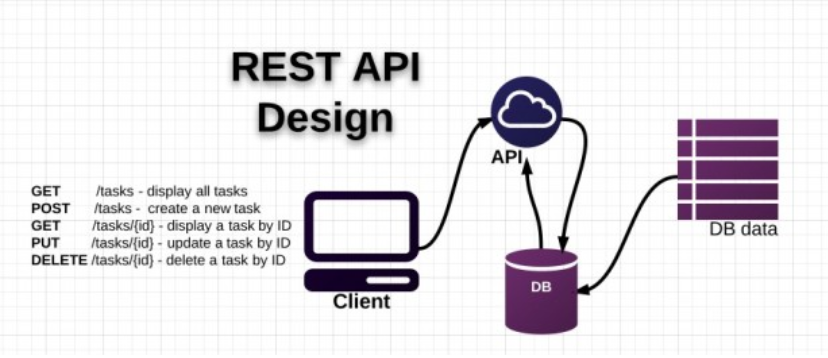
\includegraphics[width=\textwidth]{img/API.png}

\noindent{\normalsize \textbf{Diễn giải các thành phần}}
\begin{itemize}
    \item \textbf{API (Application Programming Interface):} API là một tập hợp các quy tắc và cơ chế cho phép một ứng dụng hoặc thành phần tương tác với một ứng dụng hoặc thành phần khác. API đóng vai trò như một cầu nối, giúp các ứng dụng trao đổi dữ liệu với nhau một cách dễ dàng. Dữ liệu trả về từ API thường được định dạng ở các kiểu phổ biến như JSON hoặc XML, phù hợp để tích hợp vào các ứng dụng web hoặc di động.
    
    \item \textbf{REST (REpresentational State Transfer):} REST là một kiểu kiến trúc (architectural style) được sử dụng để thiết kế API, dựa trên việc chuyển đổi trạng thái biểu diễn của tài nguyên. REST tận dụng các phương thức HTTP đơn giản như GET, POST, PUT, DELETE để thực hiện các thao tác trên tài nguyên. Thay vì sử dụng một URL để xử lý thông tin phức tạp, REST gửi các yêu cầu HTTP đến một URL cụ thể nhằm truy xuất hoặc chỉnh sửa dữ liệu, giúp giao tiếp giữa các hệ thống trở nên trực quan và hiệu quả.
    
    \item \textbf{RESTful API:} RESTful API là một tiêu chuẩn thiết kế API cho các ứng dụng web, tập trung vào việc quản lý các tài nguyên (resource) và cho phép các ứng dụng khác nhau (web, mobile, v.v.) giao tiếp với nhau. Chức năng quan trọng nhất của RESTful API là quy định cách sử dụng các phương thức HTTP (như GET để lấy dữ liệu, POST để tạo mới, PUT để cập nhật, DELETE để xóa) và cách định dạng URL để truy cập các tài nguyên. RESTful API không quy định logic mã nguồn của ứng dụng và không bị giới hạn bởi ngôn ngữ lập trình, do đó bất kỳ ngôn ngữ hoặc framework nào (như Java với Spring Boot, JavaScript với Node.js) cũng có thể được sử dụng để thiết kế một RESTful API.
\end{itemize}


